\documentclass[aspectratio=1610]{beamer}
\usepackage[utf8]{inputenc}
% \usepackage[default,oldstyle,scale=0.95]{opensans}
% \usepackage[T1]{fontenc}
\usepackage{sansmathfonts}
\usepackage[T1]{fontenc}

\usepackage[natbib=true,style=numeric,sorting=none]{biblatex}
\addbibresource{references.bib}

\usepackage{tikz}
\usepackage{pgf-pie}  
\usepackage{caption}
\usepackage{subcaption}
\usepackage{algorithm}
\usepackage{algpseudocode}
\usepackage{amsmath,amssymb,amsfonts}
\usepackage{svg}

\usetikzlibrary{arrows.meta}
\usetikzlibrary{tikzmark}
\usetikzlibrary{math}
\usetikzlibrary{backgrounds,calc,positioning}
\usepackage{qrcode}
\usepackage{siunitx}
\usetikzlibrary{patterns,positioning,arrows.meta,decorations.pathreplacing}

\usepackage{pgfplots}
\usepackage{algorithm, algpseudocode}



\usetheme{main}

\captionsetup{font=scriptsize,labelfont=scriptsize}


\title[Numerical optimization]{Numerical optimization : theory and applications}

\date[]{}
\author[AM]{\textbf{Ammar Mian} \\ \footnotesize Associate professor, LISTIC, Université Savoie Mont Blanc}

\newcommand{\red}[1]{\textcolor{red}{#1}}
% \newcommand{\alert}[1]{{\textbf{\alert{#1}}}}


%%%%%% NEW MATH DEFINITIONS %%%%%

\usepackage{amsmath,amsfonts,bm}

% Mark sections of captions for referring to divisions of figures
\newcommand{\figleft}{{\em (Left)}}
\newcommand{\figcenter}{{\em (Center)}}
\newcommand{\figright}{{\em (Right)}}
\newcommand{\figtop}{{\em (Top)}}
\newcommand{\figbottom}{{\em (Bottom)}}
\newcommand{\captiona}{{\em (a)}}
\newcommand{\captionb}{{\em (b)}}
\newcommand{\captionc}{{\em (c)}}
\newcommand{\captiond}{{\em (d)}}

% Highlight a newly defined term
\newcommand{\newterm}[1]{{\bf #1}}


% Figure reference, lower-case.
\def\figref#1{figure~\ref{#1}}
% Figure reference, capital. For start of sentence
\def\Figref#1{Figure~\ref{#1}}
\def\twofigref#1#2{figures \ref{#1} and \ref{#2}}
\def\quadfigref#1#2#3#4{figures \ref{#1}, \ref{#2}, \ref{#3} and \ref{#4}}
% Section reference, lower-case.
\def\secref#1{section~\ref{#1}}
% Section reference, capital.
\def\Secref#1{Section~\ref{#1}}
% Reference to two sections.
\def\twosecrefs#1#2{sections \ref{#1} and \ref{#2}}
% Reference to three sections.
\def\secrefs#1#2#3{sections \ref{#1}, \ref{#2} and \ref{#3}}
% Reference to an equation, lower-case.
% \def\eqref#1{equation~\ref{#1}}
% Reference to an equation, upper case
\def\Eqref#1{Equation~\ref{#1}}
% A raw reference to an equation---avoid using if possible
\def\plaineqref#1{\ref{#1}}
% Reference to a chapter, lower-case.
\def\chapref#1{chapter~\ref{#1}}
% Reference to an equation, upper case.
\def\Chapref#1{Chapter~\ref{#1}}
% Reference to a range of chapters
\def\rangechapref#1#2{chapters\ref{#1}--\ref{#2}}
% Reference to an algorithm, lower-case.
\def\algref#1{algorithm~\ref{#1}}
% Reference to an algorithm, upper case.
\def\Algref#1{Algorithm~\ref{#1}}
\def\twoalgref#1#2{algorithms \ref{#1} and \ref{#2}}
\def\Twoalgref#1#2{Algorithms \ref{#1} and \ref{#2}}
% Reference to a part, lower case
\def\partref#1{part~\ref{#1}}
% Reference to a part, upper case
\def\Partref#1{Part~\ref{#1}}
\def\twopartref#1#2{parts \ref{#1} and \ref{#2}}

\def\ceil#1{\lceil #1 \rceil}
\def\floor#1{\lfloor #1 \rfloor}
\def\1{\bm{1}}
\newcommand{\train}{\mathcal{D}}
\newcommand{\valid}{\mathcal{D_{\mathrm{valid}}}}
\newcommand{\test}{\mathcal{D_{\mathrm{test}}}}

\def\eps{{\epsilon}}


% Random variables
\def\reta{{\textnormal{$\eta$}}}
\def\ra{{\textnormal{a}}}
\def\rb{{\textnormal{b}}}
\def\rc{{\textnormal{c}}}
\def\rd{{\textnormal{d}}}
\def\re{{\textnormal{e}}}
\def\rf{{\textnormal{f}}}
\def\rg{{\textnormal{g}}}
\def\rh{{\textnormal{h}}}
\def\ri{{\textnormal{i}}}
\def\rj{{\textnormal{j}}}
\def\rk{{\textnormal{k}}}
\def\rl{{\textnormal{l}}}
% rm is already a command, just don't name any random variables m
\def\rn{{\textnormal{n}}}
\def\ro{{\textnormal{o}}}
\def\rp{{\textnormal{p}}}
\def\rq{{\textnormal{q}}}
\def\rr{{\textnormal{r}}}
\def\rs{{\textnormal{s}}}
\def\rt{{\textnormal{t}}}
\def\ru{{\textnormal{u}}}
\def\rv{{\textnormal{v}}}
\def\rw{{\textnormal{w}}}
\def\rx{{\textnormal{x}}}
\def\ry{{\textnormal{y}}}
\def\rz{{\textnormal{z}}}

% Random vectors
\def\rvepsilon{{\mathbf{\epsilon}}}
\def\rvtheta{{\mathbf{\theta}}}
\def\rva{{\mathbf{a}}}
\def\rvb{{\mathbf{b}}}
\def\rvc{{\mathbf{c}}}
\def\rvd{{\mathbf{d}}}
\def\rve{{\mathbf{e}}}
\def\rvf{{\mathbf{f}}}
\def\rvg{{\mathbf{g}}}
\def\rvh{{\mathbf{h}}}
\def\rvu{{\mathbf{i}}}
\def\rvj{{\mathbf{j}}}
\def\rvk{{\mathbf{k}}}
\def\rvl{{\mathbf{l}}}
\def\rvm{{\mathbf{m}}}
\def\rvn{{\mathbf{n}}}
\def\rvo{{\mathbf{o}}}
\def\rvp{{\mathbf{p}}}
\def\rvq{{\mathbf{q}}}
\def\rvr{{\mathbf{r}}}
\def\rvs{{\mathbf{s}}}
\def\rvt{{\mathbf{t}}}
\def\rvu{{\mathbf{u}}}
\def\rvv{{\mathbf{v}}}
\def\rvw{{\mathbf{w}}}
\def\rvx{{\mathbf{x}}}
\def\rvy{{\mathbf{y}}}
\def\rvz{{\mathbf{z}}}

% Elements of random vectors
\def\erva{{\textnormal{a}}}
\def\ervb{{\textnormal{b}}}
\def\ervc{{\textnormal{c}}}
\def\ervd{{\textnormal{d}}}
\def\erve{{\textnormal{e}}}
\def\ervf{{\textnormal{f}}}
\def\ervg{{\textnormal{g}}}
\def\ervh{{\textnormal{h}}}
\def\ervi{{\textnormal{i}}}
\def\ervj{{\textnormal{j}}}
\def\ervk{{\textnormal{k}}}
\def\ervl{{\textnormal{l}}}
\def\ervm{{\textnormal{m}}}
\def\ervn{{\textnormal{n}}}
\def\ervo{{\textnormal{o}}}
\def\ervp{{\textnormal{p}}}
\def\ervq{{\textnormal{q}}}
\def\ervr{{\textnormal{r}}}
\def\ervs{{\textnormal{s}}}
\def\ervt{{\textnormal{t}}}
\def\ervu{{\textnormal{u}}}
\def\ervv{{\textnormal{v}}}
\def\ervw{{\textnormal{w}}}
\def\ervx{{\textnormal{x}}}
\def\ervy{{\textnormal{y}}}
\def\ervz{{\textnormal{z}}}

% Random matrices
\def\rmA{{\mathbf{A}}}
\def\rmB{{\mathbf{B}}}
\def\rmC{{\mathbf{C}}}
\def\rmD{{\mathbf{D}}}
\def\rmE{{\mathbf{E}}}
\def\rmF{{\mathbf{F}}}
\def\rmG{{\mathbf{G}}}
\def\rmH{{\mathbf{H}}}
\def\rmI{{\mathbf{I}}}
\def\rmJ{{\mathbf{J}}}
\def\rmK{{\mathbf{K}}}
\def\rmL{{\mathbf{L}}}
\def\rmM{{\mathbf{M}}}
\def\rmN{{\mathbf{N}}}
\def\rmO{{\mathbf{O}}}
\def\rmP{{\mathbf{P}}}
\def\rmQ{{\mathbf{Q}}}
\def\rmR{{\mathbf{R}}}
\def\rmS{{\mathbf{S}}}
\def\rmT{{\mathbf{T}}}
\def\rmU{{\mathbf{U}}}
\def\rmV{{\mathbf{V}}}
\def\rmW{{\mathbf{W}}}
\def\rmX{{\mathbf{X}}}
\def\rmY{{\mathbf{Y}}}
\def\rmZ{{\mathbf{Z}}}

% Elements of random matrices
\def\ermA{{\textnormal{A}}}
\def\ermB{{\textnormal{B}}}
\def\ermC{{\textnormal{C}}}
\def\ermD{{\textnormal{D}}}
\def\ermE{{\textnormal{E}}}
\def\ermF{{\textnormal{F}}}
\def\ermG{{\textnormal{G}}}
\def\ermH{{\textnormal{H}}}
\def\ermI{{\textnormal{I}}}
\def\ermJ{{\textnormal{J}}}
\def\ermK{{\textnormal{K}}}
\def\ermL{{\textnormal{L}}}
\def\ermM{{\textnormal{M}}}
\def\ermN{{\textnormal{N}}}
\def\ermO{{\textnormal{O}}}
\def\ermP{{\textnormal{P}}}
\def\ermQ{{\textnormal{Q}}}
\def\ermR{{\textnormal{R}}}
\def\ermS{{\textnormal{S}}}
\def\ermT{{\textnormal{T}}}
\def\ermU{{\textnormal{U}}}
\def\ermV{{\textnormal{V}}}
\def\ermW{{\textnormal{W}}}
\def\ermX{{\textnormal{X}}}
\def\ermY{{\textnormal{Y}}}
\def\ermZ{{\textnormal{Z}}}

% Vectors
\def\vzero{{\bm{0}}}
\def\vone{{\bm{1}}}
\def\vmu{{\bm{\mu}}}
\def\vtheta{{\bm{\theta}}}
\def\va{{\bm{a}}}
\def\vb{{\bm{b}}}
\def\vc{{\bm{c}}}
\def\vd{{\bm{d}}}
\def\ve{{\bm{e}}}
\def\vf{{\bm{f}}}
\def\vg{{\bm{g}}}
\def\vh{{\bm{h}}}
\def\vi{{\bm{i}}}
\def\vj{{\bm{j}}}
\def\vk{{\bm{k}}}
\def\vl{{\bm{l}}}
\def\vm{{\bm{m}}}
\def\vn{{\bm{n}}}
\def\vo{{\bm{o}}}
\def\vp{{\bm{p}}}
\def\vq{{\bm{q}}}
\def\vr{{\bm{r}}}
\def\vs{{\bm{s}}}
\def\vt{{\bm{t}}}
\def\vu{{\bm{u}}}
\def\vv{{\bm{v}}}
\def\vw{{\bm{w}}}
\def\vx{{\bm{x}}}
\def\vy{{\bm{y}}}
\def\vz{{\bm{z}}}

% Elements of vectors
\def\evalpha{{\alpha}}
\def\evbeta{{\beta}}
\def\evepsilon{{\epsilon}}
\def\evlambda{{\lambda}}
\def\evomega{{\omega}}
\def\evmu{{\mu}}
\def\evpsi{{\psi}}
\def\evsigma{{\sigma}}
\def\evtheta{{\theta}}
\def\eva{{a}}
\def\evb{{b}}
\def\evc{{c}}
\def\evd{{d}}
\def\eve{{e}}
\def\evf{{f}}
\def\evg{{g}}
\def\evh{{h}}
\def\evi{{i}}
\def\evj{{j}}
\def\evk{{k}}
\def\evl{{l}}
\def\evm{{m}}
\def\evn{{n}}
\def\evo{{o}}
\def\evp{{p}}
\def\evq{{q}}
\def\evr{{r}}
\def\evs{{s}}
\def\evt{{t}}
\def\evu{{u}}
\def\evv{{v}}
\def\evw{{w}}
\def\evx{{x}}
\def\evy{{y}}
\def\evz{{z}}

% Matrix
\def\mA{{\bm{A}}}
\def\mB{{\bm{B}}}
\def\mC{{\bm{C}}}
\def\mD{{\bm{D}}}
\def\mE{{\bm{E}}}
\def\mF{{\bm{F}}}
\def\mG{{\bm{G}}}
\def\mH{{\bm{H}}}
\def\mI{{\bm{I}}}
\def\mJ{{\bm{J}}}
\def\mK{{\bm{K}}}
\def\mL{{\bm{L}}}
\def\mM{{\bm{M}}}
\def\mN{{\bm{N}}}
\def\mO{{\bm{O}}}
\def\mP{{\bm{P}}}
\def\mQ{{\bm{Q}}}
\def\mR{{\bm{R}}}
\def\mS{{\bm{S}}}
\def\mT{{\bm{T}}}
\def\mU{{\bm{U}}}
\def\mV{{\bm{V}}}
\def\mW{{\bm{W}}}
\def\mX{{\bm{X}}}
\def\mY{{\bm{Y}}}
\def\mZ{{\bm{Z}}}
\def\mBeta{{\bm{\beta}}}
\def\mPhi{{\bm{\Phi}}}
\def\mLambda{{\bm{\Lambda}}}
\def\mSigma{{\bm{\Sigma}}}

% Tensor
\DeclareMathAlphabet{\mathsfit}{\encodingdefault}{\sfdefault}{m}{sl}
\SetMathAlphabet{\mathsfit}{bold}{\encodingdefault}{\sfdefault}{bx}{n}
\newcommand{\tens}[1]{\bm{\mathsfit{#1}}}
\def\tA{{\tens{A}}}
\def\tB{{\tens{B}}}
\def\tC{{\tens{C}}}
\def\tD{{\tens{D}}}
\def\tE{{\tens{E}}}
\def\tF{{\tens{F}}}
\def\tG{{\tens{G}}}
\def\tH{{\tens{H}}}
\def\tI{{\tens{I}}}
\def\tJ{{\tens{J}}}
\def\tK{{\tens{K}}}
\def\tL{{\tens{L}}}
\def\tM{{\tens{M}}}
\def\tN{{\tens{N}}}
\def\tO{{\tens{O}}}
\def\tP{{\tens{P}}}
\def\tQ{{\tens{Q}}}
\def\tR{{\tens{R}}}
\def\tS{{\tens{S}}}
\def\tT{{\tens{T}}}
\def\tU{{\tens{U}}}
\def\tV{{\tens{V}}}
\def\tW{{\tens{W}}}
\def\tX{{\tens{X}}}
\def\tY{{\tens{Y}}}
\def\tZ{{\tens{Z}}}


% Graph
\def\gA{{\mathcal{A}}}
\def\gB{{\mathcal{B}}}
\def\gC{{\mathcal{C}}}
\def\gD{{\mathcal{D}}}
\def\gE{{\mathcal{E}}}
\def\gF{{\mathcal{F}}}
\def\gG{{\mathcal{G}}}
\def\gH{{\mathcal{H}}}
\def\gI{{\mathcal{I}}}
\def\gJ{{\mathcal{J}}}
\def\gK{{\mathcal{K}}}
\def\gL{{\mathcal{L}}}
\def\gM{{\mathcal{M}}}
\def\gN{{\mathcal{N}}}
\def\gO{{\mathcal{O}}}
\def\gP{{\mathcal{P}}}
\def\gQ{{\mathcal{Q}}}
\def\gR{{\mathcal{R}}}
\def\gS{{\mathcal{S}}}
\def\gT{{\mathcal{T}}}
\def\gU{{\mathcal{U}}}
\def\gV{{\mathcal{V}}}
\def\gW{{\mathcal{W}}}
\def\gX{{\mathcal{X}}}
\def\gY{{\mathcal{Y}}}
\def\gZ{{\mathcal{Z}}}

% Sets
\def\sA{{\mathbb{A}}}
\def\sB{{\mathbb{B}}}
\def\sC{{\mathbb{C}}}
\def\sD{{\mathbb{D}}}
% Don't use a set called E, because this would be the same as our symbol
% for expectation.
\def\sF{{\mathbb{F}}}
\def\sG{{\mathbb{G}}}
\def\sH{{\mathbb{H}}}
\def\sI{{\mathbb{I}}}
\def\sJ{{\mathbb{J}}}
\def\sK{{\mathbb{K}}}
\def\sL{{\mathbb{L}}}
\def\sM{{\mathbb{M}}}
\def\sN{{\mathbb{N}}}
\def\sO{{\mathbb{O}}}
\def\sP{{\mathbb{P}}}
\def\sQ{{\mathbb{Q}}}
\def\sR{{\mathbb{R}}}
\def\sS{{\mathbb{S}}}
\def\sT{{\mathbb{T}}}
\def\sU{{\mathbb{U}}}
\def\sV{{\mathbb{V}}}
\def\sW{{\mathbb{W}}}
\def\sX{{\mathbb{X}}}
\def\sY{{\mathbb{Y}}}
\def\sZ{{\mathbb{Z}}}

% Entries of a matrix
\def\emLambda{{\Lambda}}
\def\emA{{A}}
\def\emB{{B}}
\def\emC{{C}}
\def\emD{{D}}
\def\emE{{E}}
\def\emF{{F}}
\def\emG{{G}}
\def\emH{{H}}
\def\emI{{I}}
\def\emJ{{J}}
\def\emK{{K}}
\def\emL{{L}}
\def\emM{{M}}
\def\emN{{N}}
\def\emO{{O}}
\def\emP{{P}}
\def\emQ{{Q}}
\def\emR{{R}}
\def\emS{{S}}
\def\emT{{T}}
\def\emU{{U}}
\def\emV{{V}}
\def\emW{{W}}
\def\emX{{X}}
\def\emY{{Y}}
\def\emZ{{Z}}
\def\emSigma{{\Sigma}}

% entries of a tensor
% Same font as tensor, without \bm wrapper
\newcommand{\etens}[1]{\mathsfit{#1}}
\def\etLambda{{\etens{\Lambda}}}
\def\etA{{\etens{A}}}
\def\etB{{\etens{B}}}
\def\etC{{\etens{C}}}
\def\etD{{\etens{D}}}
\def\etE{{\etens{E}}}
\def\etF{{\etens{F}}}
\def\etG{{\etens{G}}}
\def\etH{{\etens{H}}}
\def\etI{{\etens{I}}}
\def\etJ{{\etens{J}}}
\def\etK{{\etens{K}}}
\def\etL{{\etens{L}}}
\def\etM{{\etens{M}}}
\def\etN{{\etens{N}}}
\def\etO{{\etens{O}}}
\def\etP{{\etens{P}}}
\def\etQ{{\etens{Q}}}
\def\etR{{\etens{R}}}
\def\etS{{\etens{S}}}
\def\etT{{\etens{T}}}
\def\etU{{\etens{U}}}
\def\etV{{\etens{V}}}
\def\etW{{\etens{W}}}
\def\etX{{\etens{X}}}
\def\etY{{\etens{Y}}}
\def\etZ{{\etens{Z}}}

% The true underlying data generating distribution
\newcommand{\pdata}{p_{\rm{data}}}
% The empirical distribution defined by the training set
\newcommand{\ptrain}{\hat{p}_{\rm{data}}}
\newcommand{\Ptrain}{\hat{P}_{\rm{data}}}
% The model distribution
\newcommand{\pmodel}{p_{\rm{model}}}
\newcommand{\Pmodel}{P_{\rm{model}}}
\newcommand{\ptildemodel}{\tilde{p}_{\rm{model}}}
% Stochastic autoencoder distributions
\newcommand{\pencode}{p_{\rm{encoder}}}
\newcommand{\pdecode}{p_{\rm{decoder}}}
\newcommand{\precons}{p_{\rm{reconstruct}}}

\newcommand{\laplace}{\mathrm{Laplace}} % Laplace distribution

\newcommand{\E}{\mathbb{E}}
\newcommand{\Ls}{\mathcal{L}}
% \newcommand{\R}{\mathbb{R}}
\newcommand{\emp}{\tilde{p}}
\newcommand{\lr}{\alpha}
\newcommand{\reg}{\lambda}
\newcommand{\rect}{\mathrm{rectifier}}
\newcommand{\softmax}{\mathrm{softmax}}
\newcommand{\sigmoid}{\sigma}
\newcommand{\softplus}{\zeta}
\newcommand{\KL}{D_{\mathrm{KL}}}
\newcommand{\Var}{\mathrm{Var}}
\newcommand{\standarderror}{\mathrm{SE}}
\newcommand{\Cov}{\mathrm{Cov}}
% Wolfram Mathworld says $L^2$ is for function spaces and $\ell^2$ is for vectors
% But then they seem to use $L^2$ for vectors throughout the site, and so does
% wikipedia.
\newcommand{\normlzero}{L^0}
\newcommand{\normlone}{L^1}
\newcommand{\normltwo}{L^2}
\newcommand{\normlp}{L^p}
\newcommand{\normmax}{L^\infty}

\newcommand{\parents}{Pa} % See usage in notation.tex. Chosen to match Daphne's book.

% \DeclareMathOperator*{\argmax}{arg\,max}
% \DeclareMathOperator*{\argmin}{arg\,min}

\DeclareMathOperator{\sign}{sign}
\DeclareMathOperator{\Tr}{Tr}
\let\ab\allowbreak


\newcommand{\mat}[1]{\mathbf{#1}}
\renewcommand{\vec}[1]{\boldsymbol{#1}}
\renewcommand{\det}[1]{\lvert #1 \rvert}
\newcommand{\Esp}[2]{\mathbb{E}_{#1}\left[#2 \right]}
\renewcommand{\v}{\vec{v}}
\newcommand{\eye}[1]{\mathbf{I}_{#1}}
\newcommand{\norm}[1]{\left\| #1 \right\|}
\newcommand{\argmin}[1]{\underset{#1}{\operatorname{argmin}}}
\newcommand{\argmax}[1]{\underset{#1}{\operatorname{argmax}}}

% \newcommand{\bm}[1]{\boldsymbol{#1}}
\def\R{{\mathbb{R}}}
\def\K{{\mathbb{K}}}
\def\C{{\mathbb{C}}}
\def\N{{\mathbb{N}}}
\def\Z{{\mathbb{Z}}}
\def\d{{\rm d}}


\def\eme{{{\grave{e}me}}}

\def\m{{\mbox{m}}}
\def\Hz{{\mbox{Hz}}}
\def\Watt{{\mbox{W}}}

\DeclareMathOperator{\vecop}{vec}
\DeclareMathOperator{\unvec}{vec^{-1}}
\DeclareMathOperator{\tr}{tr}
\DeclareMathOperator{\diag}{diag}
\DeclareMathOperator{\prox}{prox}
\DeclareMathOperator{\rank}{rank}
\DeclareMathOperator{\complexj}{\mathsf{j}}
\DeclareMathOperator{\proj}{proj}
\DeclareMathOperator{\sinc}{sinc}






\AtBeginBibliography{\scriptsize}

%%%%%%%%%%%%%%%%%%%%%%%%%%%%%%%%%%%%%%%%%%%%%%%%%%%%%%%%%%%%
%                     END OF PREAMBLE
%
%%%%%%%%%%%%%%%%%%%%%%%%%%%%%%%%%%%%%%%%%%%%%%%%%%%%%%%%%%%%

\begin{document}
%%%%%%%%%%%%%%%


  
\begin{frame}[noframenumbering,plain]
\titlepage
\end{frame}
\begingroup
\setbeamercolor{background canvas}{bg=main}
\setbeamercolor{titlelike}{fg=text-light, bg=light}
\begin{frame}[noframenumbering,plain]{Outline}
    \tableofcontents[]
\end{frame}

\endgroup

\AtBeginSection[]{
        \setbeamercolor{background canvas}{bg=main} 
    \begin{frame}[plain, noframenumbering]
        \tableofcontents[currentsection]
    \end{frame}
    \setbeamercolor{background canvas}{bg=light} 
}


\AtBeginSubsection[]
{
    \setbeamercolor{background canvas}{bg=main} 
    \begin{frame}[noframenumbering, plain, label=]
        % \frametitle{Plan}  
        \tableofcontents[currentsection,currentsubsection]
    \end{frame}
    \setbeamercolor{background canvas}{bg=light} 
}



%%%%%%%%%%%%%%%%%%%%%%%%%%%%%%%%%%%%%%%%%%%%%%%%%%%%%%%%%%%%
%%%%%%%%%%%%%%%%%%%%%%%%%%%%%%%%%%%%%%%%%%%%%%%%%%%%%%%%%%%%
\section{Introduction}

\begin{frame}{Unconstrained Optimization Context}
  \begin{block}{Our Goal}
    Starting from an initial point $\mathbf{x}_0$, generate a sequence of iterates:
    $$\{\mathbf{x}_k\}_{k=0}^{\infty}$$
    such that $f(\mathbf{x}_{k+1}) < f(\mathbf{x}_k)$ until convergence.
  \end{block}
  
  \vspace{0.3cm}
  
  \textbf{Key Question:} How do we move from $\mathbf{x}_k$ to $\mathbf{x}_{k+1}$?
  
  \vspace{0.3cm}
  
  \begin{itemize}
    \item Choose a direction $\mathbf{p}_k$
    \item Choose a step length $\alpha_k$
    \item Update: $\mathbf{x}_{k+1} = \mathbf{x}_k + \alpha_k \mathbf{p}_k$
  \end{itemize}
\end{frame}

\begin{frame}{Optimization on Level Sets}
  \begin{center}
    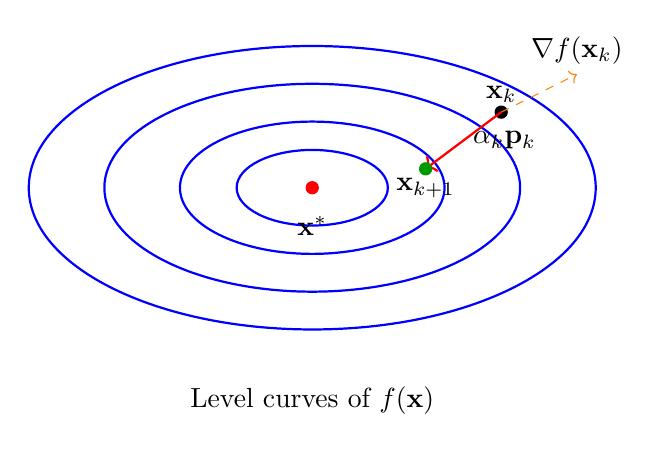
\begin{tikzpicture}[scale=1.2]
      % Draw level curves (ellipses)
      \draw[thick, blue] (0,0) ellipse (3cm and 1.5cm);
      \draw[thick, blue] (0,0) ellipse (2.2cm and 1.1cm);
      \draw[thick, blue] (0,0) ellipse (1.4cm and 0.7cm);
      \draw[thick, blue] (0,0) ellipse (0.8cm and 0.4cm);
      
      % Mark the minimum
      \fill[red] (0,0) circle (2pt);
      \node[below] at (0,-0.2) {$\mathbf{x}^*$};
      
      % Current point
      \fill[black] (2,0.8) circle (2pt);
      \node[above] at (2,0.8) {$\mathbf{x}_k$};
      
      % Direction vector
      \draw[->, thick, red] (2,0.8) -- (1.2,0.2);
      \node[right] at (1.6,0.5) {$\alpha_k \mathbf{p}_k$};
      
      % Next point
      \fill[green!60!black] (1.2,0.2) circle (2pt);
      \node[below] at (1.2,0.2) {$\mathbf{x}_{k+1}$};
      
      % Gradient direction
      \draw[->, dashed, orange] (2,0.8) -- (2.8,1.2);
      \node[above] at (2.8,1.2) {$\nabla f(\mathbf{x}_k)$};
      
      \node[below] at (0,-2) {Level curves of $f(\mathbf{x})$};
    \end{tikzpicture}
  \end{center}
\end{frame}

\section{Two Strategies: Line Search and Trust Region}

\begin{frame}{Line Search Strategy}
  \begin{block}{Line Search Approach}
    \begin{enumerate}
      \item Choose a search direction $\mathbf{p}_k$
      \item Find step length $\alpha_k$ by approximately solving:
      $$\min_{\alpha > 0} f(\mathbf{x}_k + \alpha \mathbf{p}_k)$$
      \item Update: $\mathbf{x}_{k+1} = \mathbf{x}_k + \alpha_k \mathbf{p}_k$
    \end{enumerate}
  \end{block}
  
  \vspace{0.3cm}
  
  \textbf{Key insight:} Fix direction first, then find distance.
  
  \vspace{0.3cm}
  
  \begin{itemize}
    \item Exact line search is expensive and unnecessary
    \item Use inexact line search with appropriate conditions
    \item Generate limited number of trial step lengths
  \end{itemize}
\end{frame}

\begin{frame}{Trust Region Strategy}
  \begin{block}{Trust Region Approach}
    \begin{enumerate}
      \item Build local quadratic model $m_k(\mathbf{x}_k + \mathbf{p})$
      \item Choose maximum distance $\Delta_k$ (trust region radius)
      \item Solve: $\min_{\mathbf{p}} m_k(\mathbf{x}_k + \mathbf{p})$ subject to $\|\mathbf{p}\| \leq \Delta_k$
      \item If step is successful, accept; otherwise shrink $\Delta_k$
    \end{enumerate}
  \end{block}
  
  \vspace{0.3cm}
  
  \textbf{Key insight:} Fix maximum distance first, then find best direction.
  
  \vspace{0.3cm}
  
  Quadratic model: $m_k(\mathbf{x}_k + \mathbf{p}) = f_k + \mathbf{p}^T \nabla f_k + \frac{1}{2}\mathbf{p}^T \mathbf{B}_k \mathbf{p}$
\end{frame}

\begin{frame}{Visualization of Trust region}
  \begin{center}
    
\includegraphics[height=0.9\textheight]{./figures/trust_region/main.pdf}
  \end{center}
\end{frame}

\begin{frame}{Line Search vs Trust Region}
  \begin{center}
    \begin{tabular}{|c|c|c|}
      \hline
      \textbf{Aspect} & \textbf{Line Search} & \textbf{Trust Region} \\
      \hline
      \hline
      Order of choice & Direction $\rightarrow$ Distance & Distance $\rightarrow$ Direction \\
      \hline
      Search direction & Fixed per iteration & Changes when $\Delta_k$ changes \\
      \hline
      Step acceptance & Always accept & May reject and retry \\
      \hline
      Computational cost & Lower per iteration & Higher per iteration \\
      \hline
      Robustness & Good for well-scaled problems & Better for ill-conditioned \\
      \hline
    \end{tabular}
  \end{center}
  
  \vspace{0.5cm}
  
  \textbf{Focus of this lecture:} Line search methods
\end{frame}

\section{Search Directions for Line Search Methods}

\begin{frame}{Steepest Descent Direction}
  \begin{theorem}[Steepest Descent Direction]
    The direction of steepest decrease is the solution to:
    $$\min_{\mathbf{p}} \mathbf{p}^T \nabla f_k \quad \text{subject to} \quad \|\mathbf{p}\| = 1$$
    
    \textbf{Solution:} $\mathbf{p} = -\frac{\nabla f_k}{\|\nabla f_k\|}$
  \end{theorem}
  
  \vspace{0.3cm}
  
  \begin{proof}[Proof sketch]
    Using $\mathbf{p}^T \nabla f_k = \|\mathbf{p}\| \|\nabla f_k\| \cos \theta$:
    \begin{itemize}
      \item Minimize $\cos \theta$ subject to $\|\mathbf{p}\| = 1$
      \item Minimum occurs when $\cos \theta = -1$ (i.e., $\theta = \pi$)
      \item This gives $\mathbf{p} = -\nabla f_k / \|\nabla f_k\|$
    \end{itemize}
  \end{proof}
\end{frame}

\begin{frame}{General Descent Directions}
  \begin{definition}[Descent Direction]
    A direction $\mathbf{p}_k$ is a \textbf{descent direction} if:
    $$\mathbf{p}_k^T \nabla f_k < 0$$
    
    Equivalently, the angle $\theta_k$ between $\mathbf{p}_k$ and $-\nabla f_k$ satisfies $\theta_k < \pi/2$.
  \end{definition}
  
  \vspace{0.3cm}
  
  \begin{block}{Why Descent Directions Work}
    From Taylor expansion: $f(\mathbf{x}_k + \epsilon \mathbf{p}_k) = f(\mathbf{x}_k) + \epsilon \mathbf{p}_k^T \nabla f_k + O(\epsilon^2)$
    
    If $\mathbf{p}_k^T \nabla f_k < 0$, then $f(\mathbf{x}_k + \epsilon \mathbf{p}_k) < f(\mathbf{x}_k)$ for sufficiently small $\epsilon > 0$.
  \end{block}
\end{frame}

\subsection{Step-Length Conditions}

\begin{frame}{The Step Length Tradeoff}
  \begin{block}{Fundamental Challenge}
    We want to choose $\alpha_k$ to minimize $\phi(\alpha) = f(\mathbf{x}_k + \alpha \mathbf{p}_k)$, but:
    \begin{itemize}
      \item Exact minimization is too expensive
      \item Need substantial reduction in $f$
      \item Cannot spend too much time choosing $\alpha_k$
    \end{itemize}
  \end{block}
  
  \vspace{0.3cm}
  
  \textbf{Solution:} Use inexact line search with appropriate termination conditions
  
  \vspace{0.3cm}
  
  \begin{itemize}
    \item \textbf{Sufficient decrease:} Ensure adequate reduction in $f$
    \item \textbf{Curvature condition:} Prevent steps that are too short
    \item \textbf{Bracketing + interpolation:} Efficient implementation
  \end{itemize}
\end{frame}

\subsection{The Wolfe Conditions}

\begin{frame}{Sufficient Decrease Condition (Armijo)}
  \begin{definition}[Armijo Condition]
    $$f(\mathbf{x}_k + \alpha \mathbf{p}_k) \leq f(\mathbf{x}_k) + c_1 \alpha \nabla f_k^T \mathbf{p}_k$$
    where $c_1 \in (0,1)$ (typically $c_1 = 10^{-4}$).
  \end{definition}
  
  \vspace{0.3cm}
  
  \begin{itemize}
    \item Ensures reduction proportional to step length and directional derivative
    \item Linear function $l(\alpha) = f(\mathbf{x}_k) + c_1 \alpha \nabla f_k^T \mathbf{p}_k$
    \item Since $c_1 < 1$, line $l(\alpha)$ lies above $\phi(\alpha)$ for small $\alpha$
    \item \textbf{Problem:} Satisfied by all sufficiently small $\alpha$ 
  \end{itemize}
\end{frame}

\begin{frame}{Curvature Condition}
  \begin{definition}[Curvature Condition]
    $$\nabla f(\mathbf{x}_k + \alpha_k \mathbf{p}_k)^T \mathbf{p}_k \geq c_2 \nabla f_k^T \mathbf{p}_k$$
    where $c_2 \in (c_1, 1)$.
  \end{definition}
  
  \vspace{0.3cm}
  
  \textbf{Intuition:}
  \begin{itemize}
    \item Left side is $\phi'(\alpha_k)$, right side is $c_2 \phi'(0)$
    \item If slope $\phi'(\alpha)$ is strongly negative $\Rightarrow$ can reduce $f$ more
    \item If slope is only slightly negative or positive $\Rightarrow$ terminate
  \end{itemize}
  
  \vspace{0.3cm}
  
  \textbf{Typical values:}
  \begin{itemize}
    \item $c_2 = 0.9$ for Newton/quasi-Newton methods
    \item $c_2 = 0.1$ for conjugate gradient methods
  \end{itemize}
\end{frame}

\begin{frame}{Wolfe and Strong Wolfe Conditions}
  \begin{block}{Wolfe Conditions}
    \begin{align}
      f(\mathbf{x}_k + \alpha_k \mathbf{p}_k) &\leq f(\mathbf{x}_k) + c_1 \alpha_k \nabla f_k^T \mathbf{p}_k \\
      \nabla f(\mathbf{x}_k + \alpha_k \mathbf{p}_k)^T \mathbf{p}_k &\geq c_2 \nabla f_k^T \mathbf{p}_k
    \end{align}
    with $0 < c_1 < c_2 < 1$.
  \end{block}
  
  \vspace{0.3cm}
  
  \begin{block}{Strong Wolfe Conditions}
    Replace second condition with:
    $$|\nabla f(\mathbf{x}_k + \alpha_k \mathbf{p}_k)^T \mathbf{p}_k| \leq c_2 |\nabla f_k^T \mathbf{p}_k|$$
    
    Forces $\alpha_k$ to lie near stationary points of $\phi(\alpha)$.
  \end{block}
\end{frame}

\begin{frame}{Wolfe Conditions Illustration}
  \begin{center}
    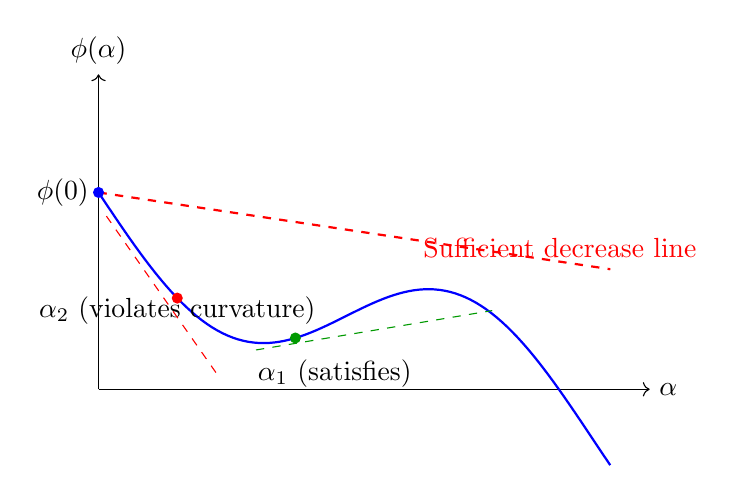
\begin{tikzpicture}[scale=1.0]
      % Define phi(alpha) = 1 - sin(alpha) - alpha/2
      \draw[->] (0,0) -- (7,0) node[right] {$\alpha$};
      \draw[->] (0,0) -- (0,4) node[above] {$\phi(\alpha)$};
      
      % Plot phi(alpha) = 1 - sin(alpha) - alpha/2
      \draw[thick, blue] plot[domain=0:6.5, samples=100] (\x, {1 - sin(\x r) - 0.5*\x + 1.5});
      
      % Plot sufficient decrease line l(alpha) = phi(0) + c1 * alpha * phi'(0)
      % phi'(0) = -cos(0) - 0.5 = -1.5, so with c1=0.1: l(alpha) = 2.5 - 0.15*alpha
      \draw[thick, red, dashed] plot[domain=0:6.5] (\x, {2.5 - 0.15*\x});
      
      % Mark phi(0)
      \fill[blue] (0,2.5) circle (2pt);
      \node[left] at (0,2.5) {$\phi(0)$};
      
      % Mark a point where curvature condition is satisfied
      \fill[green!60!black] (2.5, {1 - sin(2.5 r) - 0.5*2.5 + 1.5}) circle (2pt);
      \node[below] at (3, 0.5) {$\alpha_1$ (satisfies)};
      
      % Mark a point where curvature condition is NOT satisfied  
      \fill[red] (1.0, {1 - sin(1.0 r) - 0.5*1.0 + 1.5}) circle (2pt);
      \node[below] at (1.0, 1.3) {$\alpha_2$ (violates curvature)};
      
      % Draw tangent at alpha_1 to show curvature condition
      \draw[green!60!black, dashed] (2.0, .5) -- (5.0, 1.0);
      
      % Draw tangent at alpha_2 to show strong negative slope
      \draw[red, dashed] (0.1, 2.2) -- (1.5, 0.2);
      
      \node[right, red] at (4, 1.8) {Sufficient decrease line};
    \end{tikzpicture}
  \end{center}
\end{frame}

\begin{frame}{Existence of Wolfe Step Lengths}
  \begin{theorem}[Existence Theorem]
    Suppose $f: \mathbb{R}^n \to \mathbb{R}$ is continuously differentiable, $\mathbf{p}_k$ is a descent direction, and $f$ is bounded below along the ray $\{\mathbf{x}_k + \alpha \mathbf{p}_k \mid \alpha > 0\}$. 
    
    Then for $0 < c_1 < c_2 < 1$, there exist intervals of step lengths satisfying both the Wolfe conditions and the strong Wolfe conditions.
  \end{theorem}
  
  \vspace{0.3cm}
  
  \textbf{Key implications:}
  \begin{itemize}
    \item Wolfe conditions are not too restrictive
    \item Always possible to find acceptable step lengths
    \item Line search algorithms are well-defined
  \end{itemize}
\end{frame}

\subsection{The Goldstein Conditions}

\begin{frame}{Goldstein Conditions}
  \begin{definition}[Goldstein Conditions]
    $$f(\mathbf{x}_k) + (1-c)\alpha_k \nabla f_k^T \mathbf{p}_k \leq f(\mathbf{x}_k + \alpha_k \mathbf{p}_k) \leq f(\mathbf{x}_k) + c\alpha_k \nabla f_k^T \mathbf{p}_k$$
    with $0 < c < \frac{1}{2}$.
  \end{definition}
  
  \vspace{0.3cm}
  
  \begin{itemize}
    \item \textbf{Right inequality:} Sufficient decrease (same as Armijo)
    \item \textbf{Left inequality:} Controls step length from below
    \item Both conditions use same parameter $c$
  \end{itemize}
  
  \vspace{0.3cm}
  
  \textbf{Comparison with Wolfe:}
  \begin{itemize}
    \item (Yes) Simpler (one parameter vs two)
    \item (No) May exclude minimizers of $\phi(\alpha)$
    \item (No) Not well-suited for quasi-Newton methods
  \end{itemize}
\end{frame}

\begin{frame}{Goldstein Conditions Illustration}
  \begin{center}
    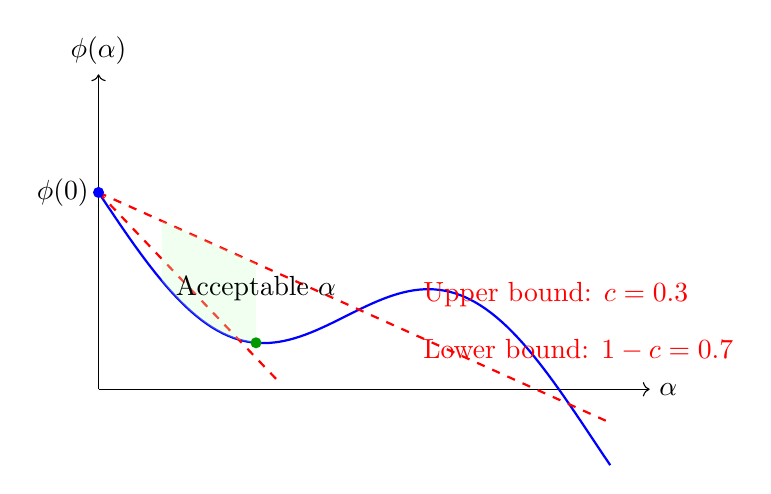
\begin{tikzpicture}[scale=1.0]
      % Define phi(alpha) = 1 - sin(alpha) - alpha/2
      \draw[->] (0,0) -- (7,0) node[right] {$\alpha$};
      \draw[->] (0,0) -- (0,4) node[above] {$\phi(\alpha)$};
      
      % Plot phi(alpha) = 1 - sin(alpha) - alpha/2
      \draw[thick, blue] plot[domain=0:6.5, samples=100] (\x, {1 - sin(\x r) - 0.5*\x + 1.5});
      
      % Plot upper bound: phi(0) + c * alpha * phi'(0) with c=0.3
      % phi'(0) = -1.5, so upper = 2.5 - 0.45*alpha
      \draw[thick, red, dashed] plot[domain=0:6.5] (\x, {2.5 - 0.45*\x});
      
      % Plot lower bound: phi(0) + (1-c) * alpha * phi'(0) with c=0.3
      % lower = 2.5 - 1.05*alpha
      \draw[thick, red, dashed] plot[domain=0:2.3] (\x, {2.5 - 1.05*\x});
      
      % Mark phi(0)
      \fill[blue] (0,2.5) circle (2pt);
      \node[left] at (0,2.5) {$\phi(0)$};
      
      % Shade acceptable region
      \fill[green!20, opacity=0.3] plot[domain=0.8:2.0] (\x, {2.5 - 0.45*\x}) --
                                   plot[domain=2.0:0.8] (\x, {1 - sin(\x r) - 0.5*\x + 1.5});
      
      % Mark acceptable points
      \fill[green!60!black] (2, {1 - sin(2 r) - 0.5*2 + 1.5}) circle (2pt);
      \node[above] at (2, 1) {Acceptable $\alpha$};
      
      \node[right, red] at (4, 1.2) {Upper bound: $c = 0.3$};
      \node[right, red] at (4, 0.5) {Lower bound: $1-c = 0.7$};
    \end{tikzpicture}
  \end{center}
\end{frame}

\subsection{Sufficient Decrease and Backtracking}

 \begin{frame}{Backtracking Line Search Algorithm}
  \begin{algorithm}[H]
    \caption{Backtracking Line Search}
    \begin{algorithmic}[1]
      \Require Choose $\bar{\alpha} > 0$, $\rho \in (0,1)$, $c \in (0,1)$
      \State Set $\alpha \leftarrow \bar{\alpha}$
      \While{$f(\mathbf{x}_k + \alpha \mathbf{p}_k) > f(\mathbf{x}_k) + c\alpha \nabla f_k^T \mathbf{p}_k$}
        \State $\alpha \leftarrow \rho \alpha$
      \EndWhile
      \State \Return $\alpha_k = \alpha$
    \end{algorithmic}
  \end{algorithm}

  \vspace{0.3cm}
  
  \textbf{Parameters:}
  \begin{itemize}
    \item $\bar{\alpha} = 1$ for Newton/quasi-Newton methods
    \item $\rho \in [0.1, 0.8]$ (contraction factor)
    \item $c = 10^{-4}$ (sufficient decrease parameter)
  \end{itemize}
  
  \vspace{0.3cm}
  
  \textbf{Termination:} Guaranteed in finite steps since $\alpha$ becomes small enough.
\end{frame}

\begin{frame}{Properties of Backtracking}
  \begin{block}{Key Properties}
    \begin{itemize}
      \item \textbf{Simplicity:} Only uses sufficient decrease condition
      \item \textbf{Efficiency:} Cheap function evaluations
      \item \textbf{Robustness:} Always finds acceptable step
      \item \textbf{Flexibility:} Can use safeguarded interpolation for $\rho$
    \end{itemize}
  \end{block}
  
  \vspace{0.3cm}
  
  \textbf{Why it works:}
  \begin{itemize}
    \item Either accepts initial step $\bar{\alpha}$ 
    \item Or finds step short enough for sufficient decrease
    \item But not too short: within factor $\rho$ of rejected step
  \end{itemize}
  
  \vspace{0.3cm}
  
  \textbf{Practical enhancement:} Use polynomial interpolation to choose $\rho$ adaptively.
\end{frame}

\section{Convergence of Line Search Methods}

\begin{frame}{Lipschitz Continuous Functions}
  \begin{columns}
    \begin{column}{0.5\textwidth}
      \begin{definition}[Lipschitz Continuity]
        A function $f: \mathbb{R}^n \to \mathbb{R}$ is \textbf{Lipschitz continuous} on a set $S$ if there exists a constant $L \geq 0$ such that:
        $$\|f(\mathbf{x}) - f(\mathbf{y})\| \leq L \|\mathbf{x} - \mathbf{y}\|$$
        for all $\mathbf{x}, \mathbf{y} \in S$.
        
        The smallest such constant $L$ is called the \textbf{Lipschitz constant}.
      \end{definition}
      
      \vspace{0.3cm}
      
      \textbf{Key Properties:}
      \begin{itemize}
        \item Lipschitz $\Rightarrow$ uniformly continuous
        \item Bounds the "steepness" of $f$
        \item If $f$ is differentiable: $L = \sup \|\nabla f(\mathbf{x})\|$
      \end{itemize}
    \end{column}
    
    \begin{column}{0.5\textwidth}
      \begin{center}
        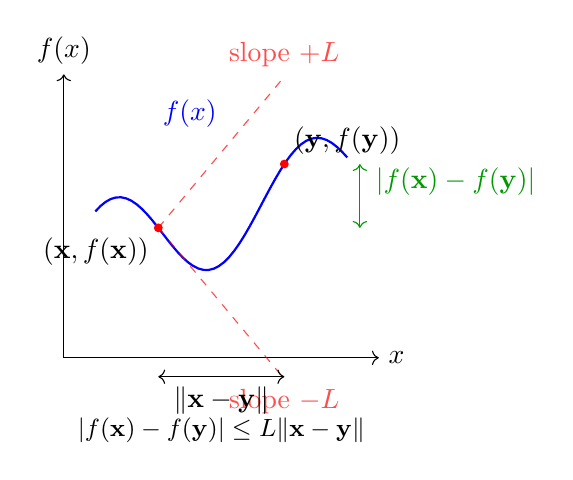
\begin{tikzpicture}[scale=0.8]
          % Axes
          \draw[->] (0,0) -- (5,0) node[right] {$x$};
          \draw[->] (0,0) -- (0,4.5) node[above] {$f(x)$};
          
          % Function curve (a wavy function that respects Lipschitz bound)
          \draw[thick, blue] plot[domain=0.5:4.5, samples=50] (\x, {1.5 + 0.8*sin(2*\x r) + 0.3*\x});
          
          % Two points on the curve
          \coordinate (A) at (1.5, {1.5 + 0.8*sin(3 r) + 0.3*1.5});
          \coordinate (B) at (3.5, {1.5 + 0.8*sin(7 r) + 0.3*3.5});
          
          \fill[red] (A) circle (2pt);
          \fill[red] (B) circle (2pt);
          \node[below left] at (A) {$(\mathbf{x}, f(\mathbf{x}))$};
          \node[above right] at (B) {$(\mathbf{y}, f(\mathbf{y}))$};
          
          % Lipschitz cone from point A
          \draw[dashed, red, opacity=0.7] (A) -- ++(2, 2*1.2) node[above] {slope $+L$};
          \draw[dashed, red, opacity=0.7] (A) -- ++(2, -2*1.2) node[below] {slope $-L$};
          
          % Distance annotations
          \draw[<->] (1.5, -0.3) -- (3.5, -0.3);
          \node[below] at (2.5, -0.3) {$\|\mathbf{x} - \mathbf{y}\|$};
          
          % Vertical distance
          \draw[<->, green!60!black] (4.7, {1.5 + 0.8*sin(3 r) + 0.3*1.5}) -- 
                                     (4.7, {1.5 + 0.8*sin(7 r) + 0.3*3.5});
          \node[right, green!60!black] at (4.8, 2.8) {$|f(\mathbf{x}) - f(\mathbf{y})|$};
          
          % Lipschitz bound illustration
          \node[below] at (2.5, -0.8) {\small $|f(\mathbf{x}) - f(\mathbf{y})| \leq L \|\mathbf{x} - \mathbf{y}\|$};
          
          % Function label
          \node[blue, above] at (2, 3.5) {$f(x)$};
        \end{tikzpicture}
      \end{center}
    \end{column}
  \end{columns}
\end{frame}

\begin{frame}{Zoutendijk's Theorem}
  \begin{theorem}[Zoutendijk's Theorem]
    Consider iterations $\mathbf{x}_{k+1} = \mathbf{x}_k + \alpha_k \mathbf{p}_k$ where $\mathbf{p}_k$ is a descent direction and $\alpha_k$ satisfies the Wolfe conditions. 
    
    Suppose $f$ is bounded below, continuously differentiable in a neighborhood of the level set $\mathcal{L} = \{\mathbf{x} : f(\mathbf{x}) \leq f(\mathbf{x}_0)\}$, and $\nabla f$ is Lipschitz continuous on $\mathcal{L}$.
    
    Then:
    $$\sum_{k \geq 0} \cos^2 \theta_k \|\nabla f_k\|^2 < \infty$$
    where $\cos \theta_k = \frac{-\nabla f_k^T \mathbf{p}_k}{\|\nabla f_k\| \|\mathbf{p}_k\|}$.
  \end{theorem}
\end{frame}

\begin{frame}{Global Convergence Result}
  \begin{corollary}[Global Convergence]
    If our method for choosing the search direction $\mathbf{p}_k$ in the iteration ensures that the angle $\theta_k$ between the negative gradient $\nabla f_k$ and the search direction $\mathbf{p}_k$ is bounded away from $90^\circ$, there exists a $\delta > 0$ such that $\cos \theta_k \geq \delta > 0 \quad \text{for all } k$.
    
    Then: $$\lim_{k \to \infty} \|\nabla f_k\| = 0$$
  \end{corollary}
  
  \vspace{0.3cm}
  
  \textbf{Applications:}
  \begin{itemize}
    \item \textbf{Steepest descent:} $\cos \theta_k = 1$
    \item \textbf{Newton:} With proper modifications 
    \item \textbf{Quasi-Newton:} With positive definite updates 
    \item \textbf{Conjugate gradient:} With restarts 
  \end{itemize}
  
  \vspace{0.3cm}
  
  \textbf{Note:} "Global convergence" = convergence to stationary points, not global minima.
\end{frame}

\section{Rate of Convergence}

\begin{frame}{Rate of Convergence}
  \begin{block}{Convergence Rates Depend on Method}
    \begin{itemize}
      \item \textbf{Steepest descent:} Linear convergence, can be very slow
      \item \textbf{Newton's method:} Quadratic convergence near solution
      \item \textbf{Quasi-Newton:} Superlinear convergence
      \item \textbf{Conjugate gradient:} Finite termination (quadratic functions)
    \end{itemize}
  \end{block}
  
  \vspace{0.3cm}
  
  \textbf{Key factors affecting rate:}
  \begin{itemize}
    \item Condition number of the Hessian
    \item Choice of search direction
    \item Quality of line search
    \item Problem structure
  \end{itemize}
  
  \vspace{0.3cm}
  
  \textbf{Reference:} Nocedal \& Wright, Chapter 3, pages 47-51 for detailed analysis.
\end{frame}


\section{Exercice}

\begin{frame}{Exercice}
  \begin{block}{Exercise: Line Search on Himmelblau Function}
    Consider the Himmelblau function:
    $$f(x,y) = (x^2 + y - 11)^2 + (x + y^2 - 7)^2$$

    We want to find minima using a line search method with the following steps:
    
    \begin{enumerate}
      \item Implement a backtracking line search algorithm to find a step length $\alpha_k$ that satisfies the Wolfe conditions.
      \item Use the steepest descent direction for the search direction $\mathbf{p}_k$.
      \item Plot the convergence path on the level sets of $f$.
    \end{enumerate}
  \end{block}
\end{frame}


\end{document}


